\section{Data, Features, Models}
% FIXME: rewrite the parts about features according to the right names
This section will mainly focus on data, features, and models.
As has been mentioned in the previous section the first key element
of machine learning is \emph{data}. Then, by processing these data,
the second main key will be extracted, the so-called \emph{features},
which are the most relevant part of the data that will be used for
learning. Finally, based on the features extracted previously, it will
be possible to build the so-called \emph{models} that will represent the
summary of the knowledge acquired through the learning process and will
be used to perform some actions.

\subsection{Learning Process}

Based on the results provided in the previous section, it is time to
introduce a more complete description of the machine learning pipeline,
as illustrated in the image below:

\vspace{5mm}

\begin{figure}[h]
      \centering
      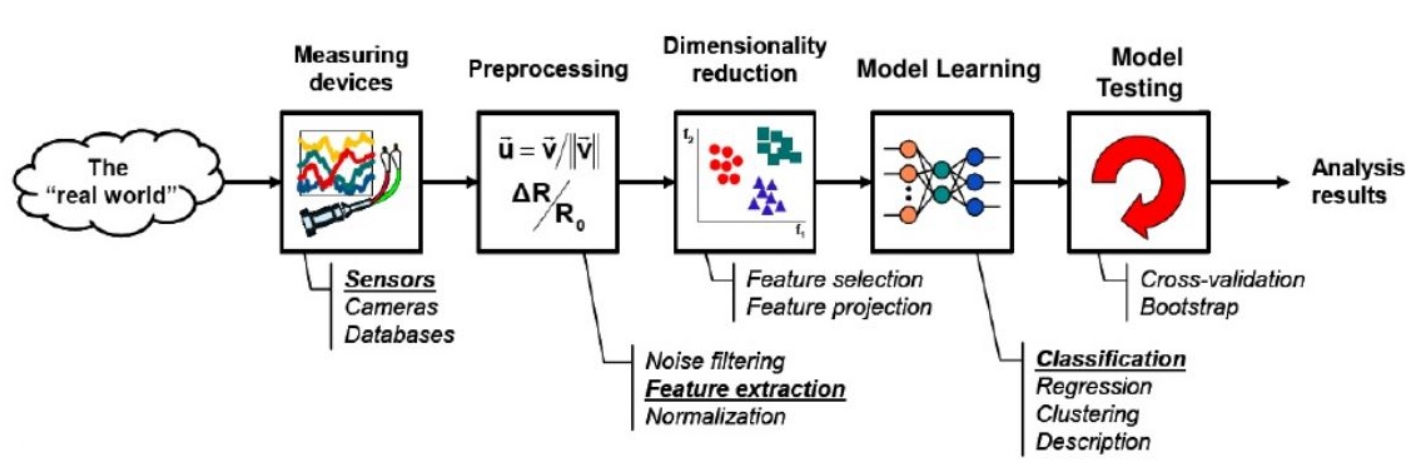
\includegraphics[width=\textwidth]{../img/Learning_process}
      \caption{Learning process in detail}
\end{figure}

\newpage

So, as can be observed in the image above, the learning process
in real-world applications where some kind of machine learning is
used is actually quite complex and it is also necessary to understand
how to perform each step of the pipeline shown below in order to build
an actually working machine learning model:

\begin{enumerate}
      \item \emph{\textbf{Data Source}}: This is the actual place where
            all data are generated. Normally this place is represented
            by the real world itself.
      \item \emph{\textbf{Data Collecting}}: This is the process by which
            all data are collected from the data source mentioned in
            point 1 by using different devices, such as
            \underline{sensors}, cameras, and databases.
      \item \emph{\textbf{Data Preprocessing}}: This is a process that
            depends on the type of the problem which is being addressed.
            Normally this process consists in some noise filtering, if the
            data are images or sensor signals, in normalization,
            if the data are seen as vectors, or in the
            so-called \emph{feature extraction}, which is achieved by
            transforming the data into a set of vectors containing relevant
            information.
      \item \emph{\textbf{Dimensionality Reduction(Optional)}}: Sometimes
            the features from the previous step are not used directly to
            produce a model, but are carefully selected to extract
            the most relevant part through the process called \emph{feature selection}.
      \item \emph{\textbf{Model Learning}}: This is the core step of the
            machine learning process in which, by applying a particular
            \emph{learning algorithm}, the actual \emph{model}
            is generated. The actual type of algorithm that will be
            applied depends on the particular nature of the problem being
            solved, such as classification, regression, clustering,
            description, and many others.
      \item \emph{\textbf{Model Testing}}: Once the model has been
            generated through a particular learning algorithm, a
            particular model testing protocol is applied to validate
            the accuracy of the generated model.
\end{enumerate}

It is also important to mention that another element that adds complexity
to the design of machine learning models is the choice of a particular
algorithm to use. This is because of the fact that there is a huge number
of machine learning algorithms that could be used. Fortunately, there is
always a guide that helps in making the right decision, that is the
particular nature of the problem to be solved.

At this point, given the general machine learning pipeline described
above, it is time to dive into the first most important element of
the process which is \emph{data}. The first
problem to solve is the fact that the concept of data is quite abstract,
but the concrete data that are used in real-world applications can be
extremely different form each other. For this reason, it is necessary to
define a general procedure that will allow representing data
independently of their actual structure. The answer to this problem is
called \emph{feature extraction}: that is the process by which each
\emph{example} in the \emph{training set} is associated with a data
structure, which is normally a simple vector of numbers with cardinality
n, that \emph{represents} the relevant information about the example and
indicates the \emph{actual form} that is seen by the algorithms. Each
such vector takes the name of \emph{feature}.

\newpage

One way of extracting these features is to consider them as
\emph{questions that can be asked} about the example, like for instance
in the image below with the fruits:

\vspace{5mm}

\begin{figure}[h]
      \centering
      \begin{subfigure}{0.40\textwidth}
            \centering
            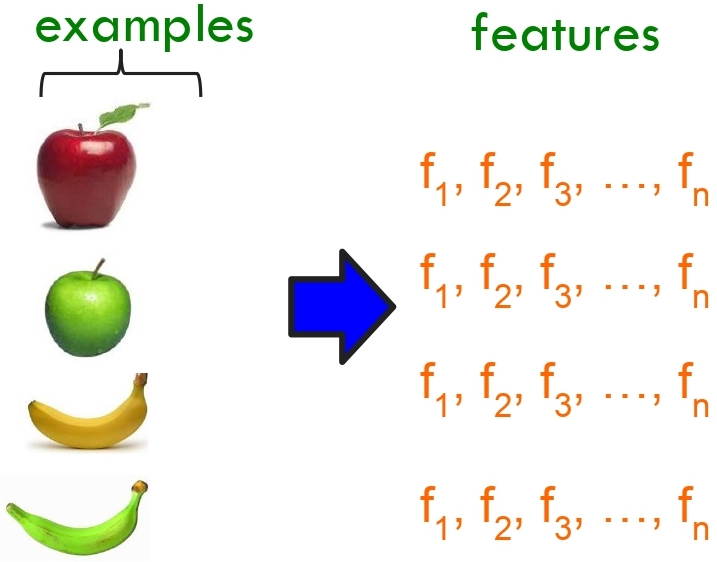
\includegraphics[width=\textwidth]{../img/Features_1}
      \end{subfigure}
      \hfill
      \begin{subfigure}{0.50\textwidth}
            \centering
            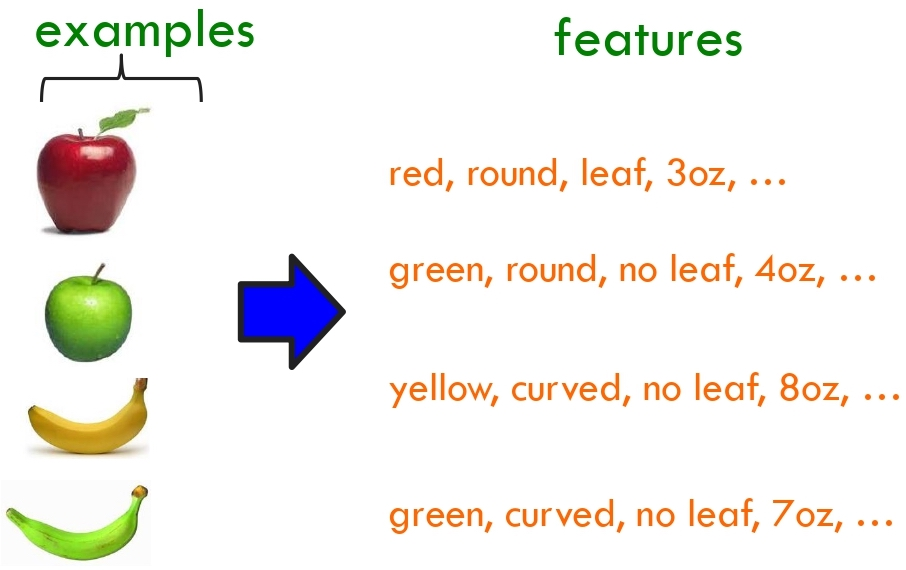
\includegraphics[width=\textwidth]{../img/Features_2}
      \end{subfigure}
      \caption{Example of features}
\end{figure}

\vspace{5mm}

Therefore, the final result of the feature extraction process is the
actual \emph{training set}, which is a set of numerical vectors, each of
which is the same dimension as the others. Unfortunately, there is a
problem with this approach, which is actually the most delicate part of
the design of the machine learning pipeline: \emph{how} are these
features chosen? There are actually many answers to this question and
the best answer should be the one that will ideally produce a set of
features that represent as well as possible the original data without
any loss of information. Therefore, there is always a risk that, after
processing the input data,
\underline{some information associated with the real data may be lost},
which in the case could cause the machine learning algorithm to work
improperly.

\subsection{Machine Learning Methods}

Now it is time to talk about different families of machine learning
methods to add a deeper understanding to what has been briefly
described in the overview subsection of these notes.

\subsubsection{Supervised Learning}

The first big family of machine learning methods is the so-called
\emph{Supervised Learning}. All methods associated with this family
have access to the data \emph{and} some annotations that are
associated with these data. These annotations are also called
\emph{labels}. Therefore, the training set, that is the input to the
learning algorithm, in these cases consists of a set of pairs, each of
which consists of an \emph{example}(in the form of a
\emph{feature vector}) and its relative \emph{label}. For this reason,
all the pairs in the training set are called \emph{labeled examples}.
Then this set of labeled examples is processed by the learning
algorithm to build a model, also called a predictor, that will be used
on new data, which have not been seen during the training phase, to
produce labels associated with these data. It is necessary to note that
all labels generated by the model will belong to the set of all possible
labels that have been learned from the training set. All this process
can be observed in the images below:

\newpage
% FIXME: resize the images below by using GIMP 

\begin{figure}[h]
      \centering
      \begin{subfigure}{0.45\textwidth}
            \centering
            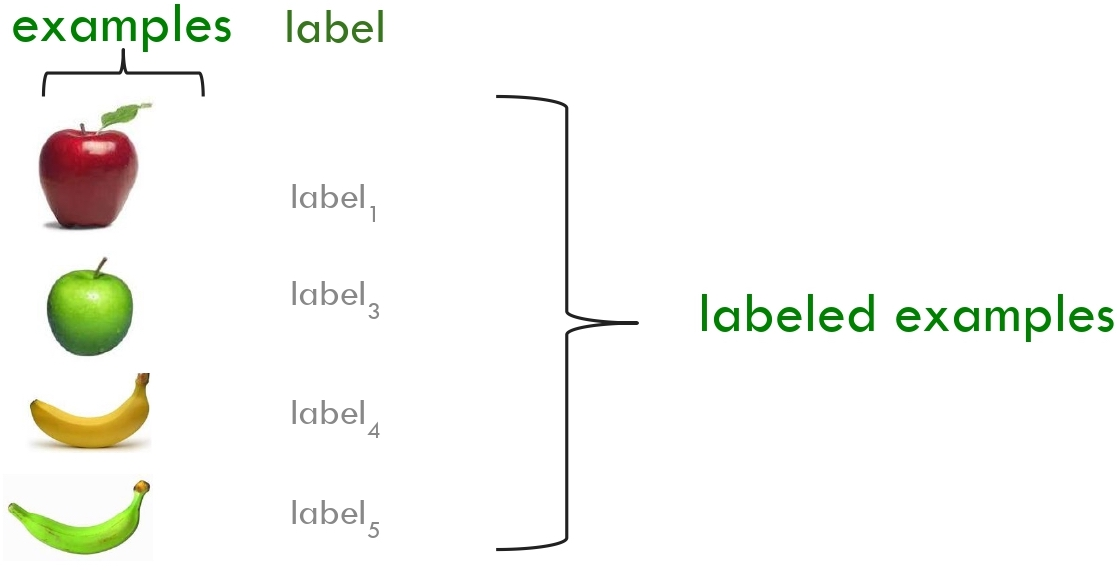
\includegraphics[width=\textwidth]{../img/Labeled_examples}
            \caption{Training Set}
      \end{subfigure}
      \hfill
      \begin{subfigure}{0.45\textwidth}
            \centering
            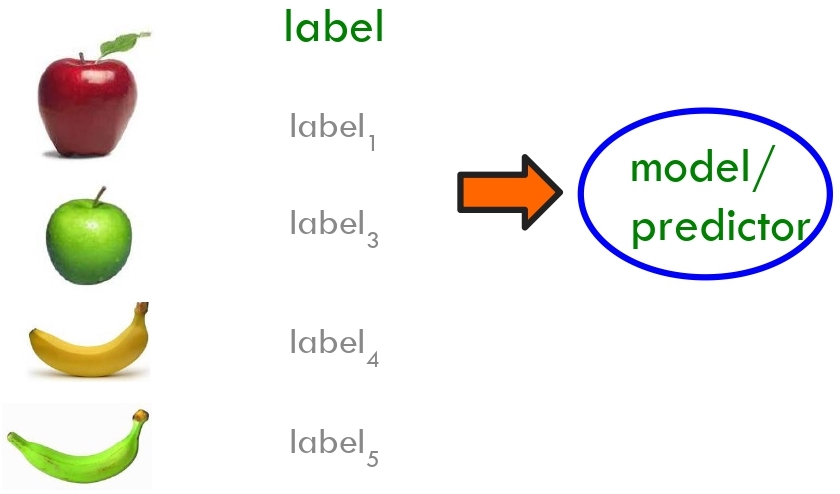
\includegraphics[width=\textwidth, height=0.55\textwidth]{../img/Supervised_training}
            \caption{Model Training}
      \end{subfigure}
      \hfill
      \begin{subfigure}{0.45\textwidth}
            \centering
            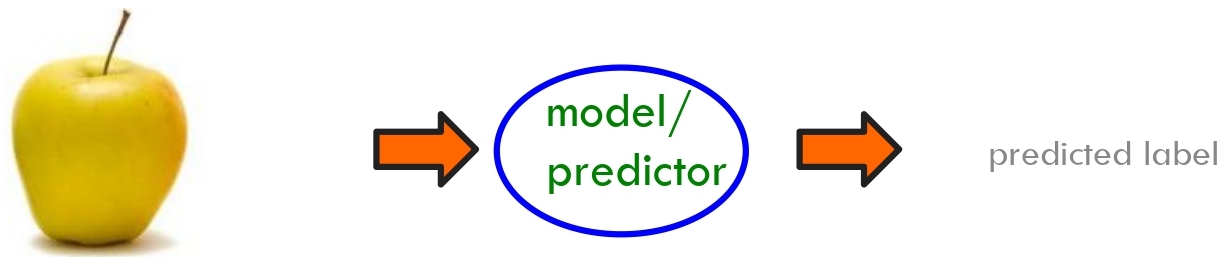
\includegraphics[width=\textwidth]{../img/Supervised_testing}
            \caption{Model Testing}
      \end{subfigure}
\end{figure}

\vspace{5mm}

At this point, it is possible to introduce some major machine learning
tasks that use the supervised learning structure defined above:

\begin{itemize}
      \item \emph{\textbf{Classification}}: Given a training set
            $\mathcal{T}=\{(x_1,y_1),...,(x_m,y_m)\}$ where
            $m$ is the total number of pairs of labeled examples,
            the task is to learn a function $f$, defined as
            $f : \mathbb{R}^d \rightarrow \{1,2,...,k\}$ where $d$
            is the dimension of the input space and $k$ is the
            \underline{finite} number of labels, to predict the label
            $y$ given the input $x$. So the dimension of the $x$
            component(feature vector) in the pairs of labeled examples
            and as input to the function $f$ is determined by the value
            of $d$, as can be observed in the examples below:

            \vspace{5mm}

            \begin{figure}[h]
                  \centering
                  \begin{subfigure}{0.52\textwidth}
                        \centering
                        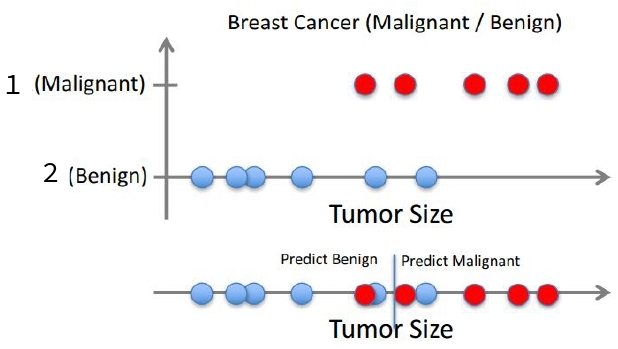
\includegraphics[width=\textwidth]{../img/Classification_1}
                        \caption{$x$ is one-dimensional($d=1$)}
                  \end{subfigure}
                  \hfill
                  \begin{subfigure}{0.38\textwidth}
                        \centering
                        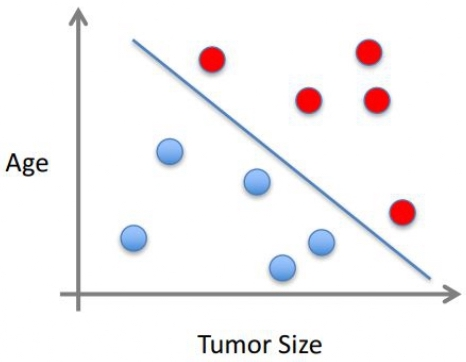
\includegraphics[width=\textwidth]{../img/Classification_2}
                        \caption{$x$ is multidimensional($d=2$)}
                  \end{subfigure}
            \end{figure}

            \vspace{5mm}

            This classification framework of supervised learning is of
            course extremely general and can be instantiated for
            several problems, such as Face Recognition, Character
            Recognition, Spam Detection, Medical Diagnosis, Biometrics
            and many others.

            \newpage

      \item \emph{\textbf{Regression}}: Given a
            training set $\mathcal{T}=\{(x_1,y_1),...,(x_m,y_m)\}$ where
            $m$ is the total number of pairs of labeled examples,
            the task is to learn a function $f$, defined as
            $f : \mathbb{R}^d \rightarrow \mathbb{R}$ where $d$
            is the dimension of the input space, to predict the label
            $y$ given the input $x$. As with Classification, the
            dimension of the $x$ component(feature vector) in the pairs
            of labeled examples and as input to the function $f$ is
            determined by the value of $d$. However, the big difference
            between Classification and Regression consists in the fact
            that all labels produced by the computed regression function
            are real-valued, so the set of all possible labels is
            \underline{not finite} by definition(i.e.\ it is
            \underline{continuous}). An example of regression is the
            following:

            \vspace{5mm}

            \begin{figure}[h]
                  \centering
                  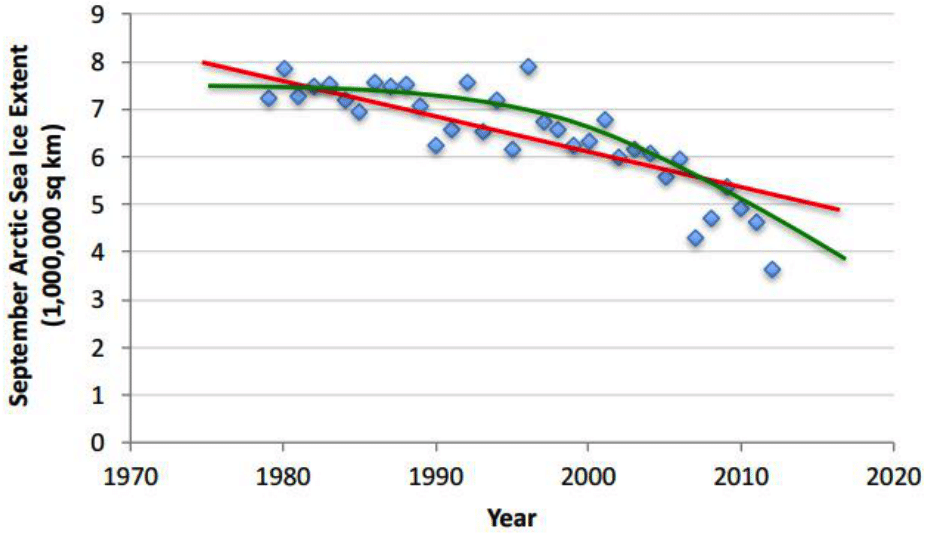
\includegraphics[width=0.7\textwidth]{../img/Regression_example}
                  \caption{Example of Regression}
            \end{figure}

            \vspace{5mm}

            As with Classification, this regression framework of
            supervised learning is of course extremely general
            and can be instantiated for several problems, such as
            Stock Value Prediction in Finance, Epidemiology, Car/Plane
            Navigation, Weather Forecasting in the area of Temporal
            Trends and many others.

      \item \emph{\textbf{Ranking}}: This is another supervised learning
            task in which all the labels in the training set and the ones
            generated by the computed ranking model are \emph{ranks},
            which are values indicating the sorting position/relevance
            of the elements. An example of ranking is search query
            evaluation in web browsers where, given a query and a set of
            web pages, a ranking is computed according to the ranks of
            the web pages, with the most relevant web sites appearing at
            the top. As with the previous two tasks, this ranking
            framework is extremely general and can be instantiated for
            several problems, such as User Preference(e.g.\ Netflix
            "My List" for movie queue ranking), Image Retrieval, Flight
            Search, Search in general and many others.
\end{itemize}

\newpage

\subsubsection{Unsupervised Learning}